\documentclass{article}
\usepackage{times}
\usepackage{lipsum}
\usepackage{graphicx}
\usepackage{mathtools}
\usepackage[margin=1.0in]{geometry}
\setlength{\parskip}{10pt plus 1pt minus 1pt}
\begin{document}
\begin{titlepage}
    \begin{center}
        \vspace*{1cm}
        \huge
        \textbf{Literature Review}
        
        \vspace{0.5cm}
        \LARGE
        Adversarial Examples in Deep Learning

        
        \vspace{1.5cm}
        
        \textbf{Rafael Carvalhaes Possas}
        
        \vfill
        
        \vspace{0.8cm}
        
        
        School of Information Technologies\\
        University of Sydney\\
        Australia\\

        
    \end{center}
\end{titlepage}
\section{Introduction}\label{sec:intro}


Artificial Intelligence efforts in the early days were focused in understanding the main principles behind human learning. For instance, recognizing digits is a trivial and effortless job for most people, however, making a computer to be able to execute this same task might not be as easy as it is for an human being. Nevertheless, by discovering the pattern behind digit recognition, computers would also be able to start understanding broader classes of images/objects \cite{krizhevsky2012}. This field of study nowadays is particularly known as "Computer Vision".

Computer Vision has Neural Networks as the underlying foundation for its algorithms. These are usually  focused in learning models that can represent certain beliefs, and through the use of what is called \textit{cost functions}, measure how well the model is actually representing the reality \cite{goodfellow2016_book}. Some of the most common machine learning tasks include: Classification, Regression and Clustering. Computer Vision problems are usually classification problems where an input image is given and an specific output class among several others is expected as a result. 

Recent advancements in computational power and the development of Deep Learning techniques helped to popularize the use of Computer Vision. Deep Learning algorithms are better represented through Convolutional Neural Networks where several layers of neurons are connected and each of these represent deep characteristics of the input data. This popularization raised some serious concerns regarding the robustness of these algorithms for executing such tasks. For instance, one would be able to attack a machine learning system in order to make it behave for his/her own benefit.

It has been shown that several machine learning models, Convolutional Neural Networks included, can misclassify adversarial images \cite{goodfellow2014}\cite{papernot2016transf}\cite{goodfellow2016}\cite{szegedy2013}. Such examples are usually created through applying small intentional perturbations to each pixel in a way that the classifier outputs the incorrect answer, while, for human beings, these perturbations do not affect the overall understanding of the desired class in most cases.

The understanding of these techniques take into account investigation on how Convolutional Neural Networks generalize. Therefore, this study will give a brief introduction to the key concepts of these algorithms before getting into the details of the adversarial examples problem. The models for adversarial creation range from simple perturbations using gradient information to black box attacks where the attacker has almost no information about the underlying architecture of the targeted system.

\section{Key Concepts}\label{sec:key_concepts}

\subsection{Neural Networks}\label{subsec:neural_deep}

Neural Networks are a class of differentiable machine learning algorithms. One can think of these networks as a set of perceptrons aligned into several layers having outputs from layer \textit{L} mapped to inputs of the layers \textit{L+1}. The output of each perceptron is named activation and the set of activations in the final layer gives the desired classification output. For instance a network could have 10 neurons in the last layer that would map to a digit classification problem using the MNIST \cite{lecun1998mnist} dataset. The neurons from 1-10 on this layer corresponds to each number, and the one with the highest activation value would be chosen as the classification output.

As most differentiable machine learning algorithms, Neural Networks models rely on optimizations of weights $\omega$ and biases $\beta$ for each set of connections between two adjacent neurons. In order to calculate these values one should  choose a cost function that measures the variance between the actual result and the desired output on each iteration of the training phase. The two methods for running this optimization algorithm on Neural Networks are known as \textit{Backpropagation} and \textit{Gradient Descent} \cite{goodfellow2016_book}. The main goal of the algorithm is to propagate small changes $\delta$ applied to any of the neurons of the network all the way to the final layer.

\begin{figure}[h!]
\centering
	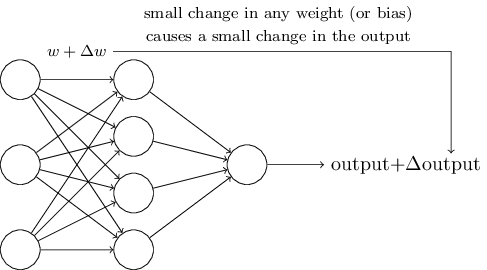
\includegraphics[scale=0.5]{net_change.png}
\caption{Output change with regards to layer(s) weight change \cite{nielsen2016}}
\label{fig:net_change}
\end{figure}

\subsection{Stochastic Gradient Descent}\label{subsec:stochastic}


The optimization problem mentioned above falls into the convex optimization category.The learning algorithm should be able to find weights and biases that best approximates the output \textit{y(x)}. This approximation consists of finding the global minimum of the chosen cost function. Different machine learning algorithms require different cost functions \cite{nielsen2016}. Neural Networks are usually have the combination of \textit{Cross-Entropy} cost function along with the \textit{Sigmoid} Neuron. Ultimately, one should be interested in calculating the change on the cost with respect to the weights and biases of all the neurons. This calculation makes use of partial derivatives with respect to the $\omega$ and $\beta$ in order to find the direction of the minimum of a function, namely gradient \cite{goodfellow2016_book}.

$$\nabla C \equiv \frac{\partial C}{\partial \omega}, \frac{\partial C}{\partial b}$$

Gradient Descent is one of the methods for finding a global/local minimum of a function. This calculation yields what is a called a gradient vector $\nabla$C which is subtracted from current weight and biases on each iteration in order to move the result towards the global or local minimum. The gradient calculation can be seen as repeatedly computing $\nabla$C, and then moving in the opposite direction "falling down" the slope of the valley.

\begin{figure}[!ht]
\centering
	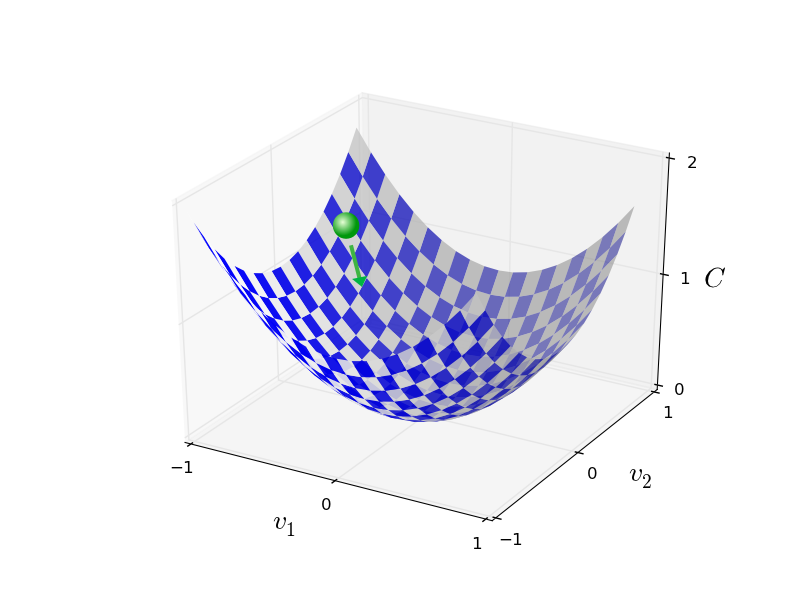
\includegraphics[scale=0.3]{valley_with_ball.png}
\caption{Gradient calculation representation \cite{nielsen2016}}
\label{fig:net_change}
\end{figure}

Convergence can be seen as reaching the valley of the aforementioned analogy. Mathematically speaking this is known as reaching a minimum of a function \cite{nielsen2016}. Some optimization problems are unable to find a global minimum due to their complexity, on this case, convergence is achieved by finding the local minimum.

The variation of this method where each iteration runs on a subset of the training input is known as \textit{Stochastic Gradient Descent}. Its biggest advantage is to speed up learning while the estimation of the gradient $\nabla$C is being computed over a subset of the data instead of all training inputs. The subset is picked randomly on every iteration and can be referred as mini-batch. These batches are selected every \textit{epoch} and the user provides how many epochs the algorithm should run. Due to the large amount of parameters, the neural networks used in Deep Learning make use of this method in order to make training to happen within feasible time ranges.

\subsection{Feedforward and Backpropagation}\label{subsec:backprop}

Feedforward is the starting point of the network weights and biases optimization.The goal is to calculate the activation of each neuron from the first layer to the output layer. It involves evaluating the sigmoid function with respect to the current weights and biases of the network by forward-propagating \textit{x} through the entire architecture. This yields the error $\delta$ used in the backpropagation algorithm.

When feedforward reaches the last layer, the error is then calculated and backpropagated to the L-1 layer. For each layer, it is needed to find the rate of change of the cost function for each weights and biases with respect to its neurons. This operation is repeated subsequently until the input layer, where the current "belief" of the network is updated making it ready for another feedforward calculation. The overall process should stop when there is no relevant changes in the output of the cost function that. This error threshold is chosen as a hyperparameter of the algorithm, and the lower the value the longer it takes to train the network.

\section{Deep Neural Networks}

Deep Neural Networks consists of several layers of connected neurons. Although efficient on accuracy, this architecture is hard to train due to its increased complexity. This complexity can be seen in image recognition tasks where the intensity value of each pixel is used as an input of the network. For instance, a 28x28 image would take 784 neurons only in the first layer, each of these would have their own $\omega$ and $\beta$.

Fully connected architectures does not take into account the inherent spatial structure of images, in other words, all pixels are treated equally. A special type of Deep Neural Networks called \textit{convolutional neural networks} can address this kind of problem with a special architecture and a faster training time \cite{krizhevsky2012}.

A convolutional neural network is different from the traditional neural network. Instead of connecting each pixel of an image, for instance, to all the neurons in the next layer, groups of pixels of fixed sizes known as patches, are connected to different groups of neurons. Each group specializes in learning specific features from the data and are not necessarily connected with all other groups in the current or next layer. The input region or group of neurons connected to a patch in the image is known as local receptive field. 

Receptive fields can be also seen as feature maps. By Sliding this field over the entire image it is possible to detect spatial features of an image.  The use of local receptive fields, shared weights and pooling makes CNN not only easier to train due to the lower number of parameters but also helps on building "deep" networks in terms features understanding \cite{zeiler2014visualizing}. The use of pooling and convolutional layers help these networks to deeply understand features of a given image while keeping state of the art accuracy and performance on classification tasks \cite{krizhevsky2012}.

\begin{figure}[!h]
\centering
	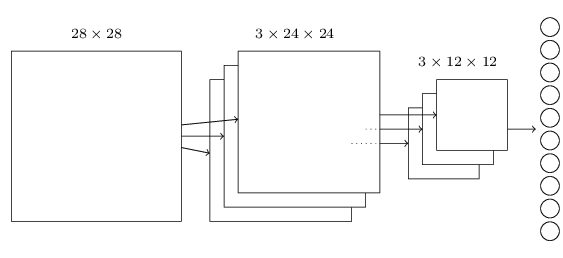
\includegraphics[scale=0.6]{conv.png}
\caption{Convolutional Neural network with image inputs, feature maps , pooling layer and output layer \cite{nielsen2016}}
\label{fig:conv}
\end{figure}

Convolutional Neural Networks have recently been seen as the best approach for computer vision problems. The archutecture developed by Krizhevsk et al. (2012) achieved an averaged top-1 and top-5 test set error rates of 37.5\% and 17\% where the previously record was 45.7\% and 25.7\% by a different technique. The network was comprised of eight layers, 5 of which were convolutional layers and the remaining were three fully connected layers. The output of the three last layers was fed to a 1000-way softmax to produce 1000 different image classes labels of the ImageNet dataset. Besides, max-pooling layers were also used following the fifth convolutional layer and response-normalization layers. Adding or removing any layers on this architecture yielded worst results. Overfitting was treated by using both Data Augmentation and Dropout \cite{hinton2012improving} techniques since the architecture had over 60 million parameters. These results show that deep convolutional networks are capable of achieving above the average results even when challenging datasets with several classes are used.

\subsection{Deep Neural Networks Properties}\label{subsec: nn_props}

Deep Neural networks can be considered models with high expressiveness that can achieve extremely good performance on computer vision tasks. At the same time that being highly expressive helps them to succeed, it also drives them to learn solutions that are not easily understandable \cite{szegedy2013}. Usually there is a discontinuity in the input-output mappings of neural networks which can lead to miss-classification of images when the network prediction error is maximized \cite{gu2014}.The learning process of these networks through the use of backpropagation is rather complex and sometimes difficult to understand.

In order to visualize the semantic meaning of individual units, studies are currently focusing on understanding the factors leading to the activation of network neurons. It has been argued that deep neural networks should be stable enough to provide robustness to small perturbation of its inputs \cite{szegedy2013}. However, it has been found by mainly Goodfellow et al. (2014) and Szegedy et al. (2013) that minimal local perturbations can indeed affect the network's predictions bringing down the assumption that DNN have very good local generalization. Methods for exploiting this vulnerability were created and proven to be effective by having a very high confidence classification of adversarial examples \cite{goodfellow2016}.

Generalization is usually achieved by making non-local assumptions of the training inputs. Deep stacks of non-linear layers are one of the ways to have the model encoding a non-local generalization prior over the input space \cite{gu2014}. Therefore, output units should be able to assign low probabilities to regions of the input space where no training examples are found within its vicinity. The representation of low-probability "pockets" of space on images can lead to the creation of Adversarial examples. These are created by adding small localized perturbations on the input space which can ultimately lead to the wrong classifier outcome. 

The following sections are going to focus on Adversarial Examples and how the exploitation of the aforementioned network properties can be used to craft such examples. Three methods will be presented along with results found by different studies. Finally, methods for using this adversarial information for regularizing networks will also be shown as a possible solution for making deep neural networks less vulnerable to these kind of attacks.

\section{Adversarial Examples}\label{sec: adversarial}

Experiments have shown that it is indeed possible to manipulate the output of a DNN algorithm \cite{nguyen2015}. Yet, they focused so far on creating models that would make adversarial examples to generalize and, thus, make deep neural networks (DNNs) to be highly susceptible to well-designed and small perturbations at the input layer \cite{gu2014}\cite{dalvi2004}.

Deep Neural Networks have been able to achieve remarkable accuracy in many classification problems \cite{krizhevsky2012}. Due to its extremely high number of non-linear units, these networks are able to automatically learn non-local generalization priors from data \cite{lowd2005}. However, some methods for creating small perturbation have recently been discovered and, therefore, put a question mark on the efficiency of these techniques.

The term transferability coined by Papernot N. et. al \cite{papernot2016transf} is one of the foundations for understanding adversarial examples in deep learning. One could slightly change a model in order to make systematic attacks to a system. These attacks range from adversarial example crafting using gradient information to black box attacks where no internal information of the algorithm is available. It is indeed feasible to transfer learning from one algorithm to another by simply querying the target with a small sample of inputs and training a local model with the resulting query dataset. This leads for learning knowledge from one algorithm being transferred to another, and, thus, the term transferability.

\begin{figure}[!h]
\centering
	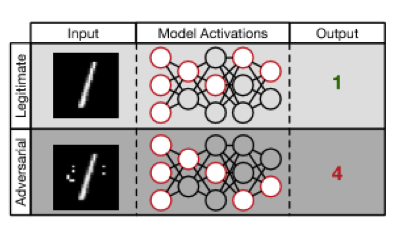
\includegraphics[scale=0.4]{transferability.png}
\caption{Small changes to an image are able to change the activation path of a Neural Network \cite{papernot2016transf}.}
\label{fig:net_change}
\end{figure}
\subsection{Fast Gradient Sign}\label{subsec:fast_gradient}

The Fast Gradient Signed method developed by Goodfellow et al. (2014) has been used as the foundation of many of the experiments in adversarial crafting. The results have led to the hypothesis that DNNs can possibly have linear behavior when in very high dimensional space.  Most inputs were miss-classified on the Goodfellow et. al \cite{goodfellow2014} experiments which shows that adversarial examples are not hard to find. The method consists on using gradient information to generate image noises that changes classification outputs.

$$ C(x + \delta)\approx C(x) + \delta * \nabla C$$

This equation aims into adding noise that emphasizes the pixels in the image with the highest importance, so the resulting perturbation can likely lead to a misclassified result. By using the \textit(sign) function of the gradient, it is assured that the value will grow linearly with the number of the dimensions \cite{goodfellow2014}. The result of many small pixel changes is likely to generate an image with a wrong label in the network output.

$$ C(x + \delta)\approx C(x) + \delta * sign(\nabla C)$$

The fast gradient sign method was able to split adversarial images in four different categories: True Adversarial, Re-focused Adversarial, Conaturally Adversarial and Benign Adversarial \cite{billovits}. True Adversarial are those given a completely different label after being perturbed. Re-Focused adversarial is the method that changes the focus of an image by giving a classification of an object that used to have lower significance while keeping the original object presence. Conaturally Adversarial are those where the new output has some close relation to the miss-classified result (e.g. Dog and Cat). Finally, Benign adversarial hapeens when neural networks misses the top prediction of the original image but the adversarial example gets classified correctly with high confidence \cite{billovits}.

\begin{figure}[!h]
\centering
	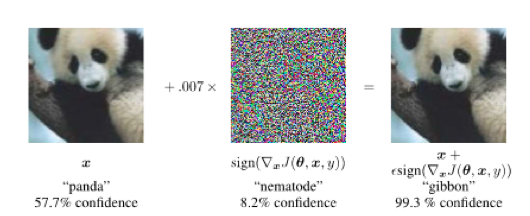
\includegraphics[scale=0.6]{panda.png}
\caption{Adversarial example crafting with fast gradient sign \cite{goodfellow2014}.}
\label{fig:net_change}
\end{figure}

\subsection{Unrecognizable Images}\label{subsec:unrec}

Studies made by Nguyen have created unrecognizable images that could have been recognized with high confidence by DNN's. The two techniques used to produce such images, namely, Gradient Ascent and Evolutionary Algorithms \cite{lecun1998gradient}\cite{floreano2008bio} were able to achieve results of over 99\% confidence on convnets using ImageNet and MNIST datasets. The use of Caffe Package \cite{jia2014caffe} along with its embedded "AlexNet"  reported 42.6\% top-1 error rate, slightly higher than previous studies \cite{krizhevsky2012}.

Generating images with the EA algorithm can be done in two different ways. Direct Encoding initializes pixels with some random noise and randomly mutates the numbers via a decreasingly probability rate for each pixel. Then, these pixels are fed into a polynomial mutation with fixed strength. Indirect Encoding is achieved through a compositional pattern-producing network (CPPN) \cite{stanley2007compositional}. The type of activation on these networks can provide geometric regularities to the resulting encoded image, thus, can help in finding underlying patterns of generated objects of the same class.

Experiments by Nguyen et. al \cite{nguyen2015} were done on both  MNIST and ImageNet datasets. On the first, less than 50 generations of direct encoding, each run of evolution repeatedly produced unrecognizable images of each digit type. By 200 generations, median confidence was around 99.99\%. The same result was repeated on the indirect encoding technique, moreover, patterns repeatedly evolved in in some digit classes characterizing that digit. However, direct encoding was less successful even after 20.000 generations evolution failed to produce high-confidence images for many categories. The median confidence was around 21.59\% although 45 classes were classified with more than 99\% confidence. Indirect encoding, on the other hand, have produced confidence scores of 88.11\%. The generated images for this methods were able to contain some features (e.g. colors) of the given class even after the CPPN generation.

The results have shown interesting properties of DNN's. They suggested that there are some unique features of images that DNN's learn and the EA algorithm can exploit. Nonetheless, it is still uncertain that different networks would learn the same features for each class.

\subsection{Black Box attacks}\label{subsec:black_box}
 
The transfer of learning knowledge from a remote algorithm to a local one makes possible an adversarial attack technique known as Black box. Even with different underlying architectures, it has been show on \cite{papernot2016transf} and \cite{papernot2016} that a local classifier can learn properties from a remote one by simply querying its outputs. Not only deep learning algorithms are vulnerable to these attacks as experiments have been done with other classes like Decision Trees, SVM, Logistic Regression and KNN.


\subsubsection{Intra-technique transferability}\label{subsubsec:intra}

The Intra-technique transferability is done by reproducing the learning process between two identical algorithms \cite{papernot2016transf}. Even though, the algorithms can differ in terms of architecture, they are still based on the same fundamental learning concept. For example, on one side there are differentiable algorithms like DNN and Logistic regressions and on the other side there are lazy learners like KNN, non-differentiable models like SVM and Decision Trees. Therefore, this technique consists of keeping the same learning method while differing the hyperparameters/architecture and using queried subset of the training data to train the local model.

In order to make a comparison between these techniques, Papernot N. et. al \cite{papernot2016transf} created five different dataset models of the MNIST to train the algorithms and compare how they perform when using different and same models of training data. All models had non-negligible vulnerability to this kind of approach. While DNN and LR were highly vulnerable to these attacks, SVM, DT and KNN were more robust achieving better overall resillience. The results have led to the hypothesis that non-differentiable techniques are more robust to black-box attacks using locally generated adversarial sample in between two algorithms of the same type \cite{papernot2016}.

\subsubsection{Cross-technique transferability}\label{subsec:intra}

The knowledge transfer between two different machine learning algorithms is known as Cross-Technique transferability. This is more complex than the method shown on section \ref{subsubsec:intra} as it involves models learned using possibly very different techniques like DNNs and DTs. Yet, this can be seen as quite strong phenomenon to which techniques like Logistic Regression, Support Vector Machines and Decision Trees along with Ensemble based models are extremely vulnerable \cite{papernot2016transf}.

Papernot N. et. al \cite{papernot2016transf} have shown a strong but heterogeneous phenomenon. While DNN's ended up as being the most robust of the methods with misclassification rates varying between 0.82\% and 38.27\%, Decision Trees were the most vulnerable with rates from 47.20\% to 89.29\%. Interesting enough, ensemble methods -- focused on measuring the output of all the "experts" in the group -- have shown quite vulnerable to the experiment. The hypothesis is that the technique explores the individual vulnerability within each of the ensemble methods.

\section{Adversarials in the Physical World}\label{sec:physical}

All the aforementioned techniques were based into feeding information directly into machine learning systems. Such model only takes into consideration situations in which attacks take place entirely within the computer. For instance, these techniques could be used by attackers to avoid spam filters or malware detectors. Even though the study is utterly relevant, a recent study conducted by \cite{goodfellow2016} have shown that it is possible to craft adversarial samples in order to perform attacks on machine learning systems which are operating in the physical world.

Although the Fast Gradient Sign method have been successful on crafting adversarial examples, there are some extensions of the method that can be used in order to create perturbations that are more likely to work in the physical world. Firstly, \cite{goodfellow2016} introduced a variation named \textit{Basic Iterative Method}. This technique consists of applying the fast method multiple times with small step sizes and making sure that all pixels are within a $\epsilon$-neighbourhood of the original image. The number of iterations was chosen heuristically with goals of being sufficient enough to have the adversarial example reaching the edge of the $\epsilon$ max-norm.

In order to perform experiments, clean photos of adversarial examples created using the three methods were taken and fed into a machine learning system using Deep Convolutional Neural Networks (Inception V3). Adversarial Images created using the "fast" method were more robust when compared to the iterative methods. The hypothesis behind the result is that iterative methods create more subtle perturbations that can be easily be destroyed by the photo transformation process (Photo Printing as described above). Overall, it could be expected that about 2/3 of the images would be top-1 misclassified and about 1/3 top-5 misclassified by the fast method using an $\epsilon$ of 16.

Adversarial examples is not only feasible on digital attacks but also on physical world scenarios. By using the correct perturbation algorithm with optimized hyperparameters one can use printed digital photos to fool day-to-day machine learning systems. As more and more machine learning is becoming part of our environment, techniques for avoiding such attacks need to be developed so these systems can become less vulnerable to any kind of attack.

\section{Adversarial Robustness of Neural Networks}\label{sec:robustness}

Good generalization is the ultimate goal of any learning technique. However, one should be able to understand when a specific model is memorizing the training set rather than learning how to generalize. Overfitting is a known problem on most algorithms and, thus, techniques like regularization were developed in order to help algorithms to achieve better results on test sets.Weight Decay is one of the most popular types of regularization where the network is penalized when large weights $\omega$ are chosen instead of small ones.

Since adversarials are exploiting intrinsic network properties, these could also be used when training a network in order to develop robustness to possible examples crafted using the same methods. By using the worst case perturbation of a point \textit{x} instead of \textit{x} itself it is possible to derive an equation that includes the perturbation within its objective function. This form of training were able to reduce the error rate of adversarial examples from 0.94\% to 0.84\% \cite{goodfellow2014}. Adversarial training can be seen as a way of teaching the model how an adversarial looks like and that it should be able to generalize not only normal images but also perturbed ones.

$$ C(\omega,x,y) = \alpha C(\omega ,x,y) + (1-\alpha )C(\omega ,x+\epsilon sign(\nabla_{x}C(\omega,x,y))$$

Another way of creating robustness was developed by using bayesian non-parametric methods. Estimating the confidence that an input is natural during the training phase can lead the network to generate priors that take into account adversarial perturbation of points \cite{billovits}. 

Since there is no information about an adversarial input to be able to infer from its distribution, Kernel Density estimation technique can be applied to the model in order to calculate the aforementioned input confidence. Nevertheless, the latter technique does not perform well in high dimensions, thus, the process of dimensionality reduction is needed so KDE can produce better estimates for the confidence levels. The use of Auto-Encoders was able to reduce the number the dimensions while keeping 68 - 72\% of the variance from a 4096 fully connected layer of VGGNET's \cite{simonyan2014very} convolutional network. The experiments of \cite{billovits} found that 80\% of images previously classified with high confidence have been mitigated using the above regularization method.
\section{Conclusion}\label{sec:conclusion}

Neural Networks have been around for almost 20 years. However, the lack of computational power and state of the art computer vision Datasets were hindering the progress of such techniques for the last years. Nowadays, the recent developments on cloud computing were responsible for making such algorithms a feasible and powerful option for image recognition tasks. Along with the popularity of Deep Learning comes also a threat. How would these systems resist to attacks and avoid any kind of leakage of sensitive information to end up in the hands of unwanted people? Fast Gradient Sign has been used as the foundation of most of the methods for adversarial example creation. This technique exploits the core of any differentiable machine learning algorithm based on convex optimization: the gradient. All studies have presented extremely high top-1 and top-5 error rates for images perturbed by this method. These results ended up exposing state of the art CNN's architecture that until now were known by their performance and robustness.

Although many examples of these threats were given, none of them focused on quantifying different images classes vulnerabilities. For instance, would an image with a noisy background be more susceptible to these attacks? This kind of study can help to understand a bit more of not only the nature of such attacks but also what kind of feature drives CNNs on the process of giving wrong class labels to perturbed image inputs. The increasingly popularity of these systems demands deeper studies on this field in order to help devising more robust techniques that can be used on day-to-day systems without posing significant threat to the community.


\pagebreak
\bibliographystyle{IEEEtran}
\bibliography{ref}





\end{document}